 \chapter{Welch's T-test} \label{chap:fobos-t-test}
 
Welch’s T-test is used as a tool for leakage assessment. This chapter describes using FOBOS to perform a fixed-vs-random t-test.
\begin{center}
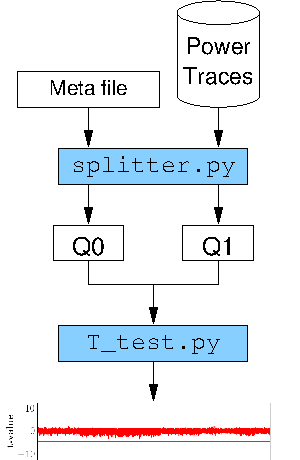
\includegraphics[scale=1]{../figures/t-test-flow}
\end{center}

\section{Background}

Usage of Welch's t-test for leakage assessment was introduced in [GOODWILL].
There are two methods to perform a t-test, specific and non-specific T-test.
In specific t-test, like DPA an intermediate bit is trageted. We perform multiple operations on the DUT using random input and power traces are collected.
The traces are then partitioned into two sets. The first set is the set of traces where the target bit equals one. 
We then run T-test on the two populations and see if they are distiguishable. This will indicate if DPA attck is likely to scucceed.
In the non-specific t-test, a fixed palintext D is selected and randomly interleaved with random data. This interleaved data is processed by the DUT and traces are collected. 
The traces are partioned into two sets, one for the fixed palintext and the other for the random. T-test is then performed on the two sets. 
If the traces are distingushable, this indicates that the device is leaking information.

The equation used in t-test is as follows [GOODWILL]:

$$
\frac{\mu_0 - \mu_1}{\sqrt{\fra\frac{s_0^2}{n_0} - \frac{s_1^2}{n_1}}}
$$

Where $\mu_0$ and $\mu_1$ are means of distributions 0 and 1, $s_0$ and $s_1$ are standard deviations, and $n_0$ and $n_1$ are the cardinality of the distributions, or the number of samples. 

\section{Test vector generation}
Fixed-vs-random t-test uses interleaved fixed and random test vectors. These vectors should be generated by the user.
We can select a fixed test vector D and create s set of test vectors that interleaves D and a randomly selected test vector. The interleaving is random.

For example the following test vector has been used to perform a t-test on an algorithm implemented on FOBOS DUT.

\begin{verbatim}
520000008300001074445161BAB57B8FFA4..6C48B60F02688701E000000043000000F0000000
52000000830000103B1C4EE0D776710B905..C2A8258DAF9BD939E000000043000000F0000000
52000000830000108EAB864A60C8CED8AC8..4B5D7CE3BBDB4666E000000043000000F0000000
5200000083000010589A762E564D5077BB3..B26D711E98989827E000000043000000F0000000
52000000830000103AEDF14E7998D7471FB..3DA0E90D53046D92E000000043000000F0000000
52000000830000106255E0D9D6FC53E0BBF..4A992A8EAF5B0646E000000043000000F0000000
52000000830000108EAB864A60C8CED8AC8..4B5D7CE3BBDB4666E000000043000000F0000000
52000000830000105E1868742DCE8785194..17EC1AE1861553D0E000000043000000F0000000
52000000830000100EEF4E5C15D888121FA..FFAED2002AC180ABE000000043000000F0000000
52000000830000108EAB864A60C8CED8AC8..4B5D7CE3BBDB4666E000000043000000F0000000
52000000830000108EAB864A60C8CED8AC8..4B5D7CE3BBDB4666E000000043000000F0000000
\end{verbatim}
\newline
A meta file specifies which trace is random and which is fixed. A one represents a random trace and a zero represents a fixed trace.
Below is an example of this file. Note how the bits correspond to random and fixed traces from the test vectors above.
\begin{verbatim}
 1101110110010011111111110101010010
\end{verbatim}



\section{T-test module cofiguration}

The T-test module needs two inputs:
\begin{enumerate}
 \item The trace file. The traces collected using the test vectors described above.
 \item The fixed vs random meta file. This file tells which trace is fixed and which trace is random.
\end{enumerate}

T-test cofiguration is loacted at \texttt{fobos/config/analysis.ini}.
Here is a sample file with explanation of each prameter:
\begin{verbatim}
[tTest]
#Number of traces to use in t-test (Both Q0 and Q1)
traceCount      = 2000
#File to store the t-t_values (output)
tValuesFile     = t_values.npy
#files to stor the distributions (random or fixed)
Q0File          = traces0.npy
Q1File          = traces1.npy
#Meta file that determines which trace is random
#and which is fixed (input). The file is expected 
#to be at fobos/sources
fvrFile         = fvrchoicefile.txt
#file to store the t-t_values vs sample no. plot (output)
\end{verbatim}

Most of the configuration parameters are file names for input and output files. The most important parameter to configure is the traceCount which is the total number of traces.
Note that the fvrchoicefile is expected to be at \texttt{/fobos/sources}. However, the trace file is in the measurement file (where the acquisition module stores it).

\section{Performing a t-test}

Run the \texttt{fobos/bin/tTest.py} script.
This will display a menu showing all the measurements done in the current project.
You can select a measurement and the t-test will be performed on it. A new analysis directroy will be created under the selected project directroy to store output files.


